\documentclass[12pt, a4paper]{article}

\usepackage{amsmath}
\usepackage{graphicx}
\usepackage{hyperref}

\begin{document}
	\author{Alex Aalbertsberg (s1008129)}	
	\title{APiE Assignment: Image Analysis}
	\maketitle
	\newpage
	\part*{Exercise 1a}
	The program can be found in the folder Exercise 1. This folder contains the following files:
	\begin{itemize}
		\item image\_analysis\_main\_routine.m: The main routine of the program. Loads the image files and calls the subsequent functions.
		\item get\_neighbors.m: A function that is used to read the values of all neighbor cells.
		\item otsu.m: A function to perform Otsu's method and return a threshold that is ideal for separating fore- and background.
		\item twopass.m: The two pass algorithm that labels each separate region for the purpose of counting the total amount of cells in the picture.
	\end{itemize}
	\newpage
	\part*{Exercise 1b}
	\begin{table}[h!]
		\centering
		\caption{Statistics of each cell}
		\resizebox{\textwidth}{!}{
		\begin{tabular}{|l|l|l|l|l|l|}
			\hline
			Area & Centroid & MajorAxisLength & MinorAxisLength & Eccentricity & Orientation \\		\hline
			1361 & {[}16.0220426157237,35.6774430565760{]} & 76.0773440696603 & 31.8383205364225 & 0.908217087274676 & -79.9837439871336 \\ \hline
			172  & {[}29.2790697674419,6.44186046511628{]} & 17.8279900107096 & 13.6771400634698 & 0.641441084849966 & -34.7965253452684 \\ \hline
			334  & {[}44.6317365269461,12.9550898203593{]} & 28.5179936096824 & 15.5144297550240 & 0.839070638058259 & 72.9037545227552  \\ \hline
			61   & {[}63.8196721311475,3.08196721311475{]} & 14.4120013542932 & 6.14352760774471 & 0.904591932430755 & -3.00313727969136 \\ \hline
			454  & {[}80.7400881057269,15.5881057268722{]} & 35.2533991936082 & 17.5046492948945 & 0.868015034443493 & 82.8406185461947  \\ \hline
			226  & {[}103.292035398230,7.76548672566372{]} & 22.3625410094315 & 14.7072611197165 & 0.753302694468095 & -41.6464505814613 \\ \hline
			295  & {[}123.267796610170,10.8406779661017{]} & 23.8879896339818 & 17.3614346825469 & 0.686864931245947 & -77.7070611489900 \\ \hline
			168  & {[}141.434523809524,8.04761904761905{]} & 18.3819646413730 & 12.9797800873535 & 0.708097220746205 & 84.1794689040105  \\ \hline
			99   & {[}159.474747474748,3.96969696969697{]} & 16.0205020269172 & 8.71579508898480 & 0.839059234613343 & -6.22016013128147 \\ \hline
			454  & {[}175.114537444934,21.8942731277533{]} & 33.2181661778477 & 18.9395882337771 & 0.821535372646975 & -77.2357989711971 \\ \hline
			444  & {[}61.5720720720721,26.6216216216216{]} & 37.6729330496012 & 17.3079597681732 & 0.888215571264737 & -86.6396845003952 \\ \hline
			507  & {[}154.601577909270,29.4536489151874{]} & 42.3420707631871 & 17.7972050218990 & 0.907376095536742 & 89.2963675474623  \\ \hline
			441  & {[}98.8412698412698,35.1723356009070{]} & 36.2861386178424 & 16.6055397230447 & 0.889143942002236 & -81.9586064912828 \\ \hline
			311  & {[}116.932475884244,35.8456591639871{]} & 30.6319509320148 & 14.0068547184257 & 0.889331569329527 & -85.3693676278098 \\ \hline
			709  & {[}135.912552891396,52.7658674188999{]} & 60.9396175181216 & 17.8249378356821 & 0.956265022260525 & -84.5845715548677 \\ \hline
			469  & {[}42.7398720682303,45.0959488272921{]} & 31.1544300580299 & 21.4990013923553 & 0.723734555502880 & -83.2330828399279 \\ \hline
			422  & {[}77.8838862559242,53.2772511848341{]} & 39.8354693272264 & 15.1937267056061 & 0.924405145627075 & 88.2905773719716  \\ \hline
			445  & {[}175.858426966292,55.5617977528090{]} & 39.6700949806903 & 18.0733185996942 & 0.890189469658375 & -77.2309052753213 \\ \hline
			481  & {[}61.0748440748441,70.7089397089397{]} & 41.9767547456275 & 17.5118921743965 & 0.908823557496212 & -82.0918068259116 \\ \hline
			378  & {[}94.5740740740741,69.4550264550265{]} & 34.8859008856194 & 16.3570223049916 & 0.883266122210345 & 88.7307719794854  \\ \hline
			399  & {[}115.395989974937,67.8671679197995{]} & 31.3355534900753 & 18.1349333779278 & 0.815516755875991 & -84.3590583636416 \\ \hline
			434  & {[}157.792626728111,69.4884792626728{]} & 33.3329033270915 & 18.9026132208405 & 0.823658785596298 & -87.6800808265478 \\ \hline
			140  & {[}3.16428571428571,69.7285714285714{]} & 28.5173943877715 & 6.66225940094624 & 0.972327760647617 & 89.4995596922104  \\ \hline
			447  & {[}40.1387024608501,80.1319910514541{]} & 37.1263371817235 & 17.3450759380024 & 0.884156625481205 & 87.7208732343748  \\ \hline
			516  & {[}17.0968992248062,90.6589147286822{]} & 36.0392562302655 & 21.9088466542249 & 0.794001214735730 & -87.0438519755254 \\ \hline
			431  & {[}170.883990719258,95.5127610208817{]} & 37.7190120178742 & 17.0894613460533 & 0.891473480727980 & 79.1002281392793  \\ \hline
			538  & {[}82.4832713754647,99.5724907063197{]} & 38.3591029049886 & 21.2131441257523 & 0.833171559224664 & -88.2503586070207 \\ \hline
			443  & {[}127.230248306998,99.6207674943567{]} & 41.9482204069698 & 18.0935508257901 & 0.902193947370075 & 79.6861470749456  \\ \hline
			421  & {[}105.961995249406,102.304038004751{]} & 39.4654910029333 & 17.4870329287118 & 0.896473771145522 & 81.9983274390859  \\ \hline
			420  & {[}147.530952380952,101.988095238095{]} & 37.8356028796452 & 18.2947308646376 & 0.875326595173378 & 78.1219198078570  \\ \hline
			52   & {[}2.11538461538462,97.5961538461538{]} & 18.0592750607845 & 4.24434424218681 & 0.971989819526562 & 86.8135612974837  \\ \hline
			487  & {[}57.9281314168378,107.616016427105{]} & 37.9954144033448 & 19.3815707291216 & 0.860113388262126 & -88.7542636306469 \\ \hline
			492  & {[}33.5203252032520,118.833333333333{]} & 38.4187223858306 & 17.9649021106090 & 0.883935944579393 & 76.3830017650481  \\ \hline
			600  & {[}9.90000000000000,127.588333333333{]} & 39.5136330848771 & 19.5370064916794 & 0.869213406285541 & 88.4479520729875  \\ \hline
			437  & {[}162.375286041190,132.951945080092{]} & 37.5329828725487 & 18.6790119043718 & 0.867366880388827 & -84.1825231473102 \\ \hline
			206  & {[}181.218446601942,134.383495145631{]} & 36.5162006712693 & 8.45437043127839 & 0.972829234112529 & -89.3519952772427 \\ \hline
			504  & {[}70.9662698412698,137.285714285714{]} & 40.8753231507958 & 17.2243223984273 & 0.906881000333857 & 74.7072089118776  \\ \hline
			439  & {[}117.451025056948,136.776765375854{]} & 37.8018395596920 & 19.2718221644430 & 0.860285984172673 & -88.2550041210044 \\ \hline
			441  & {[}93.0884353741497,135.918367346939{]} & 32.1560315896771 & 18.8409757420485 & 0.810366342848989 & 88.9655932387840  \\ \hline
			460  & {[}138.591304347826,137.993478260870{]} & 34.9009130521490 & 19.5454364983772 & 0.828474688321474 & 88.6020545397192  \\ \hline
			545  & {[}48.0146788990826,145.286238532110{]} & 39.5786228785729 & 19.9200362952657 & 0.864110047980102 & 85.7284590191609  \\ \hline
			1059 & {[}30.8980169971671,171.207743153919{]} & 67.0780423364684 & 28.9916205489965 & 0.901774271743686 & -69.8962768702647 \\ \hline
			296  & {[}5.15202702702703,165.212837837838{]} & 35.4873744048240 & 11.0601283008843 & 0.950192456765739 & -87.1559493959632 \\ \hline
			524  & {[}83.8625954198473,168.517175572519{]} & 38.1593380120294 & 19.7293611049800 & 0.855969832131060 & -86.3460616509114 \\ \hline
			488  & {[}151.536885245902,168.911885245902{]} & 39.9894393694816 & 19.9043985594211 & 0.867325500063882 & 80.7090430927396  \\ \hline
			551  & {[}105.898366606171,170.874773139746{]} & 40.1296434734146 & 19.1073039386789 & 0.879369820894250 & 86.2497232732737  \\ \hline
			469  & {[}175.441364605544,170.769722814499{]} & 37.2196387367644 & 20.1658655738931 & 0.840502847056870 & -89.1416894628186 \\ \hline
			469  & {[}128.948827292111,175.494669509595{]} & 48.0100157120600 & 16.6396531467519 & 0.938017786206689 & 84.6653446119586  \\ \hline
			572  & {[}61.1153846153846,179.110139860140{]} & 44.2589805985394 & 17.7572035126232 & 0.915985527202257 & 82.7202425988648  \\ \hline
			251  & {[}16.1673306772908,192.764940239044{]} & 20.4220796373813 & 17.2892656272406 & 0.532234905337910 & -26.7996098845513 \\ \hline
			165  & {[}76.0484848484849,194.381818181818{]} & 15.2836112685937 & 14.9055152695859 & 0.221054994440353 & 9.96105695289708  \\ \hline
			162  & {[}143.123456790123,194.777777777778{]} & 17.1876698957036 & 13.9609469423263 & 0.583288237196940 & 0.425411788351913 \\ \hline
			183  & {[}166.491803278689,194.469945355191{]} & 21.5574638277054 & 13.3438390292369 & 0.785399433620894 & -10.3729440731012 \\ \hline
			131  & {[}94.7251908396947,195.496183206107{]} & 14.2494923209649 & 12.3769425520026 & 0.495534394077327 & 3.39572849515499  \\ \hline
			126  & {[}114.746031746032,195.365079365079{]} & 14.8669685137459 & 12.3313701751253 & 0.558584649166802 & 17.7020679794304  \\ \hline
		\end{tabular}}
	\end{table}
	
	\begin{figure}[bp!]
		\caption{Fitted ellipses}
		\centering
		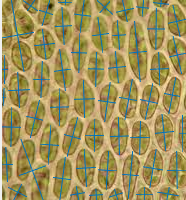
\includegraphics[width=\textwidth]{pictures/1b_fitted_ellipses}
	\end{figure}
	\newpage
	\part*{Exercise 2a}
	The program to calculate the cross-correlations can be found in the folder Exercise 2. The function that implements the cross-correlation can be found in the file named xcorr2impl.m. The execution of the assignment can be found in the file named ex2.m.
	\part*{Exercise 2b}
	Figures 2 and 3 show the autocorrelation of each pattern, i.e. the correlation they have towards themselves. The resulting plot shows a peak at a lag of zero, which is normal for autocorrelation.
	\begin{figure}[bp!]
		\caption{3D Plot of autocorrelation of pattern 1.}
		\centering
		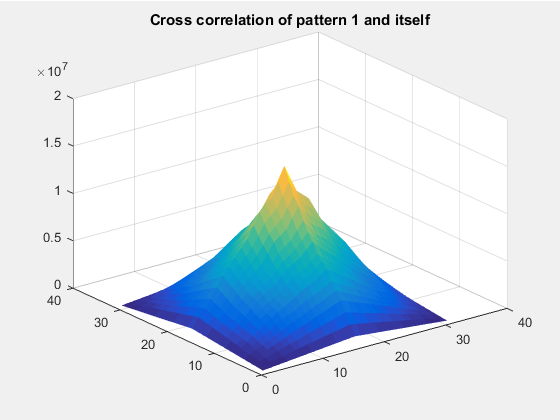
\includegraphics[width=\textwidth]{pictures/2b_pattern1}
	\end{figure}
	\begin{figure}[bp!]
		\caption{3D Plot of autocorrelation of pattern 2.}
		\centering
		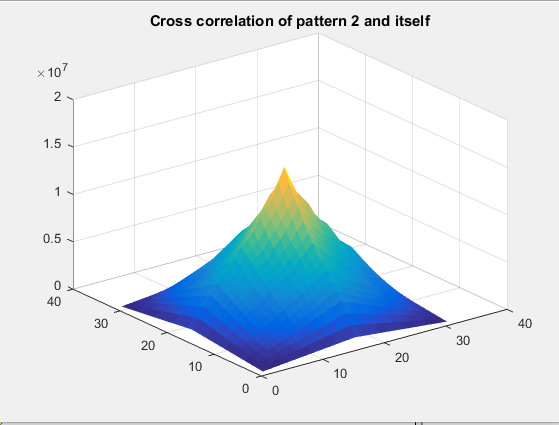
\includegraphics[width=\textwidth]{pictures/2b_pattern2}
	\end{figure}
	\newpage
	\part*{Exercise 2c}
	\begin{figure}[bp!]
		\caption{3D Plot of cross-correlation of patterns 1 and 2.}
		\centering
		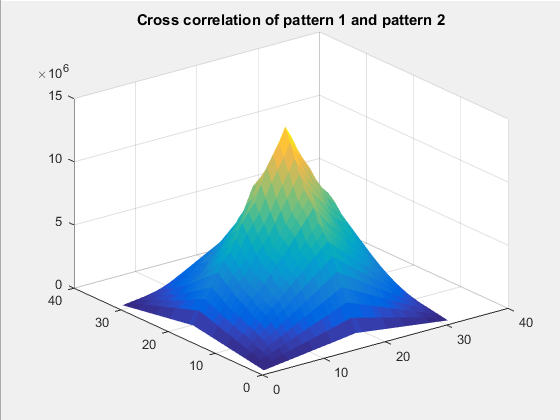
\includegraphics[width=\textwidth]{pictures/2c_pattern1xpattern2}
	\end{figure}
	\newpage
	\part*{Exercise 2d}
	The cross-correlation implementation I used originally did not calculate any displacement. When using the normalized cross-correlation (normxcorr2), the displacement is shown with offsets x = 8 and y = -7.	
\end{document}